\chapter{Stato dell'arte}
%%%%%%%%%%%%%%%%%%%%%%%%%%%%%%%%%%%%%%%%%imposta l'intestazione di pagina
\lhead[\fancyplain{}{\bfseries\thepage}]{\fancyplain{}{\bfseries\rightmark}}
\pagenumbering{arabic}
\section{La tecnologia Blockchain}
%‘‘’’
Una Blockchain (letteralmente \textit{‘‘catena di blocchi’’}) è un registro pubblico e distribuito di transazioni effettuate fra partecipanti di una rete, e rientra nella famiglia delle tecnologie ‘‘Distributed Ledger’’ (che vuol dire appunto \textit{Registro Distribuito}). Si tratta di un registro che non viene mantenuto da un unica autorità centrale (come ad esempio una banca), ma ciascun partecipante della rete (ovvero, ciascun \textit{nodo}) mantiene una copia identica del registro. Come si può intuire dal nome, la Blockchain è una struttura dati costituita da una catena di blocchi. Questi blocchi contengono una lista di transazioni avvenute in un certo arco di tempo, e sono interconnessi fra loro attraverso l'uso della crittografia. Oltre alle transazioni, ciascun blocco infatti contiene il codice hash del blocco che lo precede nella catena. Prima di essere aggiunto alla catena, un blocco deve essere approvato da un certo numero di nodi attraverso un meccanismo di consenso. Una volta accordatisi sul nuovo blocco, ciascun nodo aggiorna la propria copia del registro.

\subsection{Bitcoin e la prima blockchain}

La prima blockchain venne introdotta nel 2008, con la pubblicazione del whitepaper \textit{‘‘Bitcoin: A Peer-to-Peer Electronic Cash System’’}, da parte di una persona (o un gruppo di persone) sotto lo pseudonimo di Satoshi Nakamoto. Nakamoto, usando un insieme di tecnologie preesitenti, creò Bitcoin, una moneta elettronica basata su di un sistema completamente decentralizzato, che non deve affidarsi a nessuna autorità centrale per l'emissione di valuta o per la validazione delle transazioni. Bitcoin consiste in:
\begin{itemize}
    \item Una rete peer-to-peer decentralizzata
    \item Un registro pubblico delle transazioni (la blockchain)
    \item Un insieme di regole per la validazione indipendente delle transazioni e per l'emissione di valuta (le regole del consenso)
    \item Un meccanismo per raggiungere un consenso decentralizzato globale all'interno della rete sulla blockchain valida (l'algoritmo Proof-of-Work).
\end{itemize}L'algoritmo di consenso PoW è stata senza dubbio l'innovazione chiave. Con l'algoritmo di consenso PoW, Bitcoin risolve elegantemente quello che è stato uno dei problemi principali delle monete elettroniche fino a quel momento, il \textit{double spend}, ovvero quando la stessa unità di valuta può essere spesa in due o più transazioni differenti. L'invenzione di Nakamoto è anche una soluzione pratica al cosiddetto \textit{‘‘Problema dei Generali Bizantini’’}, ovvero il problema di accordarsi sul corso degli eventi, o sullo stato di un sistema, scambiando informazioni attraverso una rete non affidabile e potenzialmente compromessa. 

Un'altra componente importante di Bitcoin è senz'altro l'uso della crittografia. Come già detto infatti, ciascun blocco contiene al suo interno l'hash del blocco precedente (o \textit{parent block}), e questa costituisce una componente chiave della sicurezza del Bitcoin. Difatti, un algoritmo di hashing produce sempre lo stesso esatto codice hash per lo stesso input, e una qualsiasi modifica dell'input produce un risultato completamente diverso. Dunque, se un attaccante provasse a modificare un blocco, questo cambiamento si rifletterebbe nel suo codice hash. Questo causerebbe un cambiamento a catena nei blocchi successivi, che dovrebbero essere ricalcolati. Dal momento che questo richiederebbe un'enorme potenza di calcolo (e dunque consumo di energia), l'esistenza di una lunga catena rende i blocchi più vecchi \textit{immutabili}. Inoltre, gli utenti della rete Bitcoin possiedono una coppia di chiavi crittografiche, che consente loro di provare il possesso di Bitcoin all'interno della rete. Con queste chiavi, gli utenti possono firmare transazioni per "sbloccare" una certa somma e spenderla, trasferendola ad un'altro utente.

La rete Bitcoin, avviata nel 2009, utilizza dunque la blockchain come registro pubblico distribuito delle transazioni che avvengono fra i partecipanti alla rete. Col tempo tuttavia, si cominciarono a intravedere possibili utilizzi per le blockchain che andassero oltre le criptovalute. A questo punto dunque ci si iniziò a domandare se fosse possibile costruire qualcosa di nuovo sopra Bitcoin o se invece fosse necessaria la creazione di una nuova blockchain. Costruire su Bitcoin significava essere soggetti a diverse limitazioni, dunque per avere più libertà e flessibilità, costruire una nuova blockchain era l'unica opzione, nonostante richiedesse comunque un carico di lavoro considerevole.

\subsection{Ethereum, la blockchain general-purpose}

Verso la fine del 2013, Vitalik Buterin, un giovane programmatore e appassionato di criptovalute, pubblicò un whitepaper che delineava l'idea di una blockchain \textit{turing-completa} e \textit{general-purpose}. Successivamente, insieme a Gavin Wood, iniziò a lavorare a questa idea, finché nel 2015 venne lanciata Ethereum, una blockchain General-Purpose. Come altre blockchain, Ethereum ha una criptovaluta nativa chiamata Ether. ETH è una moneta digitale, molto simile al Bitcoin. A differenza di Bitcoin però, Ethereum può fare è programmabile, il che significa che gli sviluppatori possono usarla per creare nuovi tipi di applicazioni. Queste applicazioni decentralizzate (dette anche \textit{DApp}, abbreviazione per \textit{Decentralized Applications}) sfruttano i vantaggi delle criptovalute e della tecnologia blockchain. 

La base per le DApp su Ethereum sono gli \textit{smart contract}. Uno smart contract è fondamentalmente un \textit{accordo digitale}, che viene eseguito in maniera automatica. Questo implica che qualsiasi processo che richiede un interazione manuale fra due parti può essere automatizzato, senza il bisogno di un intermediario. Questo potrebbe portare alla cosiddetta ‘‘smart economy’’ in cui processi manuali soggetti ad errore vengono rimpiazzati da procedimenti automatici, completamente trasparenti ed affidabili. 

\subsubsection{Il concetto di token}

Molte delle DApp costruite su Ethereum hanno la propria criptovaluta. In altre parole, ciascuna applicazione ha il proprio ‘‘token’’: Per interagire con una di queste applicazioni, l'utente ha bisogno di acquistare il token nativo della DApp. Generalmente parlando, un token rappresenta qualcosa di specifico in un particolare ecosistema. Questo qualcosa potrebbe essere valore economico, un dividendo, un diritto di voto, ecc. Insomma, davvero qualsiasi cosa.

\subsubsection{Lo standard di base per i token: ERC 20}

ERC-20 definisce un’interfaccia standard che rappresenta un token. Lo standard fornice una serie di regole comuni che tutti i token sulla rete Ethereum possono seguire per produrre i risultati attesi. In pratica l'ERC-20 consente agli sviluppatori di risparmiare tempo nella creazione di un progetto, in quando non bisogna continuamente reinventare il modo in cui token svolgono funzioni basilari quali  i trasferimenti o il recupero di dati. Inoltre, ERC-20 consente l'interazione in maniera fluida con altri smart contracts e applicazioni decentralizzate sulla blockchain Ethereum. 

\subsubsection{ERC 721: Token non fungibili}

I token definiti attraverso lo standart ERC-20 sono token \textit{fungibili}, nel senso che ciascun token è insterscambiabile. Lo standard ERC721 invece definisce un interfaccia per token \textit{non-fungibili} (Non-Fungible tokens o NFTs) ovvero token unici nel loro genere, che pertanto non sono interscambiabili. I NFTs consentono di rappresentare attraverso un token il possesso di dati arbitrari, incrementando in maniera drastica le possibilità di ciò che può essere rappresentato come un Token sulla Blockchain Ethereum. Ciascun NFT è legato ad un identificativo univoco, che rende ciascun token unico per il suo proprietario.

Il concetto di Token non fungibile si può applicare con facilità ad ogni tipo di oggetto collezionabile. Di fatto, i NFTs hanno creato una nuova infrastruttura per giochi basati sulla blockchain. Un esempio famoso è sicuramente il progetto CryptoKitties, un gioco che permette di comprare, vendere e scambiare carte virtuali che rappresentano CryptoKitty. Ciascun CryptoKitty è completamente unico nel suo genere, e viene rappresentato da un token non-fungibile. Lanciato nel 2017, questo gioco è stato il pioniere nell'uso dei token non fungibili per rappresentare oggetti collezionabili, e ha provato che le persone attribuiscono valore ad \textit{oggetti digitali scarsamente disponibili} (\textit{digitally-scarce goods}). Difatti, Il valore di un singolo token può raggiungere cifre molto alte (anche più di 100mila dollari), e ad oggi sono stati scambiati CryptoKitties per un valore complessivo superiore a 27 milioni di dollari.

\section{Limiti delle Blockchain: Scalabilità}

Vi è sicuramente un grosso entusiasmo attorno ad Ethereum e alle blockchain in generale. Dall'applicazione esclusiva al campo delle criptovalute, si è passati, nel giro di pochi anni, da un utilizzo delle blockchain eslcusivamente nel campo delle criptovalute, alla prospettiva di un utilizzo delle blockchain nei più svariati ambiti: alcuni esempi potrebbero essere il campo della sanità, la protezione del copyright o le votazioni elettroniche. In futuro si ipotizza quindi una diffusione crescente di questa tecnologia. Tuttavia, uno dei problemi ormai noti delle blockchain, che costituisce un limite a tale diffusione è quello della loro bassa scalabilità. Per scalabilità si intende la capacità di un sistema di supportare un volume crescente di lavoro aggiungendo risorse al sistema stesso. Chiaramente, un'adozione della blockchain su scala globale porterebbe certamente ad avere un utenza sempre maggiore e di conseguenza un volume di transazioni molto più alto. Per come è stata progettata, la blockchain possiede poca scalabilità, e dunque l'aumento del carico di lavoro che si prospetta in futuro non sarebbe attualmente supportabile.

La scalabilità delle blockchain è complicata perché, per come questa tecnologia è stata progettata, è richiesto che ciascun nodo mantenga l'intero stato e processi ogni singola transazione che venga registrata sull'intera rete. Mentre ciò garantisce un livello molto alto di sicurezza, al tempo stesso limita notevolmente la scalabilità, poiché così facendo, una blockchain può processare tante transazioni quante ne può processare un singolo nodo. Dunque, principalmente per questo motivo, Bitcoin è limitato a circa 3-7 transazioni al secondo, mentre Ethereum a circa 7-15. Per avere un esempio numerico, si pensi che Facebook può gestire circa 175,000 richieste al secondo, il che vuol dire che Ethereum, al suo livello massimo di performance, è comunque almeno 10,000 volte più lento rispetto a Facebook. 
Solitamente si fa riferimento al problema della scalabilità come \textit{scalability trilemma}. Secondo questo trilemma, non è possibile avere un sistema che sia completamente decentralizzato, consistente e scalabile allo stesso tempo, ma è necessario un \textit{tradeoff}: si possono scegliere al massimo due di queste proprietà. Il trilemma può essere visualizzato graficamente nella forma di un triangolo \textit{DCS}.

\begin{figure}
    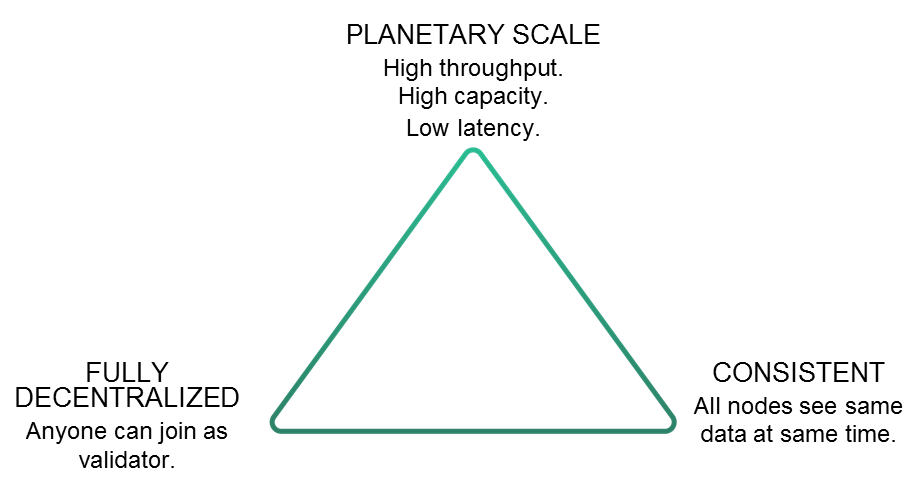
\includegraphics[width=\linewidth]{images/dcs-triangle.png}
    \caption{DCS Triangle}
    \label{fig:dcs_triangle}
\end{figure}

Per la communitiy di Ethereum, ricercatori e sviluppatori, la scalabilità costituisce probabilmente la sfida principale da risolvere per permettere alle applicazioni basate sulla blockchain di raggiungere un adozione di massa. Attualmente esistono due percorsi principali che sono stati studiati per incrementare la scalabilità delle blockchain. Da un lato si cerca di costruire dei protocolli al di sopra della blockchain base (chiamati \textit{protocolli di livello 2}) senza cambiarne la struttura, che implicano l'invio di gran parte delle transazioni su catene secondarie. Dall'altro lato si cercano soluzioni che migliorino il design della blockchain di base, e una possibile soluzione da questo punto di vista è quella di utilizzare lo \textit{sharding}.

\subsection{Sharding}

Lo sharding (letteralmente \textit{frammentazione}) è un concetto di lunga data nel campo dei sistemi distribuiti. Si parla di sharding quando un grande database viene partizionato in database più piccoli, in modo tale che i nodi del sistema distribuito debbano operare solo su una porzione del database, piuttosto che sull'interno database.
Effettuare lo sharding  della blockchain significa semplicemente partizionare la catena principale in catene più piccole e più veloci, rendendo il sistema complessivo più scalabile. Il modo per farlo sarebbe dividere lo stato e la storia delle transazioni sulla catena principale in partizioni più piccole chiamate \textit{shard}. Ad esempio, uno schema di Sharding su Ethereum potrebbe realizzare uno shard per tutti gli indirizzi che iniziano con 0x00, uno per quelli che iniziano con 0x01 e così via. 

Nella forma più semplice di sharding, ciascuno shard ha la propria storia di transazioni, e l'effetto delle transazioni in uno shard ha un effetto solo sullo shard stesso. In forme più avanzate di sharding esiste una qualche forma di comunicazione tra uno shard e l'altro (\textit{cross-shard}), dove una transazione all'interno di uno shard può generare eventi all'interno di altri shard.

Attualmente, Ethereum sta lavorando alla realizzazione dello sharding, ed ha rilasciato una \textit{roadmap}, che elenca tutte le fasi che dovrebbero portare allo sharding della blockchain Ethereum. Esistono però anche altri progetti che utilizzano lo sharding per ottenere scalabilità. E' il caso di Radix DLT.

\section{Radix DLT}

Radix DLT è una nuova piattaforma DLT (\textit{Decentralized Ledger Technology}) che si propone come alternativa alle blockchain classiche come Bitcoin o Ethereum, realizzata per essere scalabile fin dal principio e per consentire la costruzione di applicazioni su di essa con facilità. E' bene sottolineare che Radix è una tecnologia DLT, ma non si basa sulla Blockchain (quest'ultima infatti altro non è che l'implementazione più famosa di una DLT), ed utilizza un design completamente nuovo.

Radix utilizza un nuovo algoritmo di consenso chiamato Cerberus, basato su un algoritmo BFT (\textit{Byzantine Fault Tolerant}) \textit{three-phase commit} e sullo sharding per creare un sistema sicuro e scalabile. Attualmente, il progetto (diventato recentemente open source) è ancora in fase di sviluppo, e non è ancora disponibile una rete pubblica.

\subsection{Un po' di storia}

La storia di Radix inizia nel 2013, quando il suo creatore, Dan Hughes, iniziò ad eseguire una serie di test per verificare quali fossero i limiti della scalabilità di Bitcoin. Il massimo che riuscì ad ottenere da questi test fu un numero di transazioni per secondo (\textit{Transactions Per Second} o \textit{TPS}) fra 700 e 1,000. Si tratta di cifre molto basse, sapendo che, ad esempio, Visa era in grado di processare circa 24,000 TPS. 

Dan, da questo punto in poi, tentò di percorrere diverse strade per aumentare il throughput di transazioni, talvolta riuscendoci, a scapito però della sicurezza. Dopo alcuni tentativi infruttuosi, Dan teorizzò ciò che divenne il primo nucleo di Radix, ovvero il registro decentralizzato Tempo. Tempo ha una struttura basata sullo sharding, che raggruppa fra di loro le transazioni correlate e separa quelle non correlate, ed utilizza un meccanismo di consenso basato sui \textit{Logical Clock} di Lesie Lamport (un meccanismo semplice per costruire un ordine parziale e relativo degli eventi). Dan iniziò quindi a cercare membri per formare un team, che iniziò a lavorare su Tempo, sulla costruzione della rete Radix e sul Radix Engine, cioè il livello applicativo di Radix (in sostanza, la parte con la quale interagiscono gli sviluppatori). 

\subsection{Un milione di transazioni al secondo}

Tutto questo lavoro portò a compiere un test che replicò per intero tutte le transazioni avvenute su Bitcoin dal momento della sua creazione, durante il quale il sistema raggiunse la velocità di 1M di TPS Questo fu certamente un grosso traguardo per Dan e il suo team, dimostrando l'enorme scalabilità ottenibile grazie a Tempo. Tuttavia, in seguito emersero delle vulnerabilità che esponevano Tempo a due possibili vettori di attacco. Il primo è stato ribattezzato dagli sviluppatori di Radix \textit{‘‘Weak Atom Problem’’}. Esso consiste in una situazione in cui un piccolo gruppo di nodi può creare una situazione in cui il consenso è sufficientemente debole da permettere di influenzare transazioni già concluse. Il secondo vettore di attacco era invece attraverso un \textit{attacco Sybil}. Tempo infatti usava un nuovo meccanismo per proteggersi da questo tipo di attacco, chiamato \textit{Mass}, che aumentava la reputazione dei nodi all'interno della rete per la loro buona condotta nel corso del tempo. Tuttavia, è emerso che Mass non avesse grande valore per i nodi onesti, e questo apriva la strada ad un possibile mercato secondario, dove attori malevoli avrebbero potuto acquistare reputazione  (attraverso Mass) per un valore inferiore al vero.

Nonostante gli sforzi del team per cercare di risolvere questi problemi, nessuna soluzione valida venne trovata. Per questo motivo, Tempo è stato abbandonato (anche se solo in parte) e la pubblicazione di una rete pubblica Radix, inizialmente prevista per la fine del 2019, è stata spostata in data da definirsi. Al momento della scrittura di questa tesi (Febbraio/Marzo 2020), il team è al lavoro su un nuovo algoritmo di consenso, chiamato \textit{Cerberus}. In particolare, in data 3 Marzo 2020, è stato pubblicato il whitepaper su Cerberus. 

\subsection{L'architettura di Radix}

\subsubsection{Radix Engine}

\subsubsection{Cerberus}

Cerberus, ossia l'algorigmo di consenso usato da Radix, si basa sullo stesso concetto di avere uno \textit{shard space} predefinito come Tempo, ma al tempo stesso si basa su una serie di strumenti crittografici ben collaudati, che gli forniscono forti garanzie per quanto concerne la sicurezza. Attualmente, di Cerberus sappiamo che utilizza un meccanismo di consenso BFT (\textit{Byzantine Fault Tolerant}) \textit{three-phase commit}, e che utilizzerà la Proof-of-Stake (PoS) come meccanismo di guardia contro attacchi Sybil. 

\subsection{Strumenti per gli sviluppatori}

Radix DLT offre agli sviluppatori interessati a creare applicazioni che interagiscano con il registro distribuito di Radix due librerie: una libreria Java e una libreria JavaScript, entrambe ancora in versione beta. Non essendovi una rete pubblica, per testare le librerie è necessario comunicare con la rete di testing, la \textit{BETANET}, che può essere anche emulata in ambiente locale. Per questa tesi ho deciso di utilizzare la libreria JavaScript per realizzare una piccola applicazione che presenterò nei prossimi capitoli.

\subsection{Libreria JavaScript}

La libreria JavaScript Radix è costruita per essere eseguita sia client side che server side. E' costruita interamente utilizzando TypeScript, permettendo agli sviluppatori di costruire applicazioni più robuste sfruttando il \textit{type checking}. Inoltre, tale libreria segue il paradigma \textit{reactive programming}, e si appoggia alla libreria RxJS.

\subsubsection{Concetti fondamentali}

Le librerie di Radix si basano su una serie di astrazioni, raggruppate in un modello chiamato \textit{atom model}. I concetti fondamentali sono i seguenti:
\begin{itemize}
    \item \textit{Universe}: Il concetto di Universe rappresenta la rete Radix. Attualmente sono disponibili diversi Universe di testing ai quali connettersi. Essendo Radix basato sullo sharding, ciascun Universe è segmentato in un certo numero di shards.
    \item \textit{Atom}: Un Atom rappresenta tutti gli eventi che si verificano all'interno di un Universe, e che hanno l'effetto di lo stato del registro. Ciascun atom contiene al suo interno almeno un \textit{enpoint address} di destinazione.
    \item \textit{Address}: Un Address risiede su un particolare Shard, e costituisce punto di partenza e punto di arrivo per qualunque Atom nel Radix Universe. Si tratta di un riferimento ad un particolare Account, e permette ad un utente di ricevere fondi e/o dati sulla rete ad altri utenti. Gli indirizzi Radix vengono generati partendo da una chiave pubblica e da un checksum dell'Universe. 
    \item \textit{Account}: Un Account rappresenta tutti i dati salvati sul ledger per un particolare utente. Questi dati possono essere i token in possesso dell'utente, assieme ad altri dati arbitrari. Un account ha una serie di \textit{account systems}, nei quali vengono salvati gli atom ricevuti dall'account. Gli account system di default sono:
    \begin{itemize}
        \item \textit{Il Transfer System}, che mantiene una lista delle transazioni in cui è coinvolto l'account, così come il saldo dell'account per tutti i differenti tipi di token.
        \item \textit{Il Radix Messaging System}, che gestire le diverse chat di messaggistica Radix a cui l'account partecipa.
        \item \textit{Il Data System}, usato per dati personalizzati salvati sul ledger.
        \item \textit{Token Definition System}, usato per gestire i token definiti dall'utente.
    \end{itemize}
    E' possibile accedere ai dati di questi sistemi attraverso l'utilizzo di mappe ES6, oppure è possibile effettuare l'iscrizione (\textit{subscribe}) ad un \textit{subject} RxJS, che emetterà un aggiornamento ogni volta che un sistema riceve un nuovo atom dalla rete.
    \item \textit{Identity}: Un'Identity è una chiave privata associata ad un certo account, che può essere usata per firmare atom e per leggere dati criptati.
    \item \textit{Transaction Builder}: Il Transaction builder è il componente della libreria che si occupa di creare ed inviare alla rete qualsiasi tipo di Atom che il ledger radix possa accettare. Gli Atom che si possono creare con il transaction builder sono:
    \begin{itemize}
        \item \textit{Transfer Atom}: realizza il trasferimento di un item (e.g. valuta) ad un certo indirizzo.
        \item \textit{Payload Atom}: contiene dati inviati ad uno o più indirizzi.
        \item \textit{Radix Message Atom}: contiene un messaggio (caso particolare di payload atom).
        \item \textit{Mint Atom}: effettua il \textit{minting} (cioè la creazione) di una quantità specificata di token.
        \item \textit{Burn Atom}: effettua il \textit{burning} (cioè, in sostanza, l'eliminazione) di una quantità specificata di token.
    \end{itemize}
\end{itemize}
Le librerie offrono anche le funzionalità necessarie per definire dei token personalizzati. I token definiti dall'utente possono essere \textit{single-issuance} o \textit{multi-issuance}: i token multi-issuance, di cui si può fare il minting dopo la creazione, mentre i token single-issuance sono limitati all'importo specificato nella definizione del token.

\subsubsection{Radix Wallet}

Radix offre anche il software Desktop Wallet, un'applicazione che l'utente può utilizzare per memorizzare la propria identity. Il Wallet inoltre offre all'utente un interfaccia da cui:è
\begin{itemize}
    \item Controllare il saldo del proprio account.
    \item Inviare token ad un altro account.
    \item Avviare una chat di messaggistica istantanea con un altro account.
    \item Richiedere token di test all'account Faucet.
\end{itemize}